%	Auteur: Surdez Quentin
%	Titre:	 Étudiant MCT
%	Date: Mai 2022
%	Sujet: Rapport de projet P2213	
%============================================================
\documentclass[
	a4paper,									% paper format
	11pt,										% fontsize
	twoside,									% double-sided
	openright,									% begin new chapter on right side
	notitlepage,									% use no standard title page
	parskip=half,								% set paragraph skip to half of a line
]{scrreprt}										% KOMA-script report
%---------------------------------------------------------------------------

\raggedbottom
\KOMAoptions{cleardoublepage=plain}						%Add header and footer on blank pages

%Load Standard Packages: 
%---------------------------------------------------------------------------
\usepackage[standard-baselineskips]{cmbright}				%Fonts for math equation
\usepackage[french]{babel}							%French hyphenation
%\usepackage[latin1]{inputenc}  					% Unix/Linux - load extended character set (ISO 8859-1)
%\usepackage[applemac]{inputenc}
%\usepackage[ansinew]{inputenc}  					% Windows - load extended character set (ISO 8859-1)
%\usepackage[utf8]{inputenc}							%Translate input in latex language
\usepackage[T1]{fontenc}							%Allow a good hyphenation with accentuated language
%\usepackage{tgbonum}
\usepackage{ae}									%Allow vectorial letters
\usepackage{lmodern}
\usepackage{fancyhdr}								%Allow manipulation on headers and tops
\usepackage{graphicx}								%Integration of images
\usepackage{float}									%Better integration of floating objects(tables, etc)
\usepackage{caption}								%For captions of figures and tables
\usepackage{booktabs}								%Nicer tables
\usepackage{tocvsec2}								%Means of controlling the sectional numbering
\usepackage{verbatim}								%Integration of source code
\usepackage{moreverb}								%Extension of verbatim
\usepackage{listings}								%Integration of code in LATEX 
\usepackage{multirow}								%Tables with multiple rows
\usepackage{pdfpages}						
\usepackage{pst-all}								%Better handling of texts and images
\usepackage{mathrsfs}
\usepackage{colortbl}
\usepackage{listings}
\usepackage{minted}								%Better colorizing of source code WARNING need to be set up correctly according to the documentation http://tug.ctan.org/macros/latex/contrib/minted/minted.pdf
\usemintedstyle{rainbow_dash}
\usepackage{ragged2e}
\captionsetup{font=small}
\usepackage{siunitx}
\usepackage{wrapfig}
\usepackage{pgfplots}


\sisetup{
    round-mode      = places, %Round numbers
    round-precision = 2, % to 2 places
}

\usepackage{booktabs}



\newcolumntype{R}[1]{>{\raggedleft\arraybackslash }b{#1}}
\newcolumntype{L}[1]{>{\raggedright\arraybackslash }b{#1}}
\newcolumntype{C}[1]{>{\centering\arraybackslash }b{#1}}		%Adding new column types

%---------------------------------------------------------------------------

%Load Math packages
%---------------------------------------------------------------------------
\usepackage{amsmath}                    				   	% various features to facilitate writing math formulas
\usepackage{amsthm}                       	 				% enhanced version of latex's newtheorem
\usepackage{amsfonts}                      					% set of miscellaneous TeX fonts that augment the standard CM
										
\usepackage{amssymb}							% mathematical special characters
\usepackage{exscale}							% mathematical size corresponds to textsize
\usepackage{listings}
\usepackage{tikz,pgfplots}
\usepackage{array}
%---------------------------------------------------------------------------

%QR Code
%---------------------------------------------------------------------------
\usepackage{qrcode}
\usepackage{subcaption}							%Add sub-caption easily
%---------------------------------------------------------------------------

% Package to facilitate placement of boxes at absolute positions
%---------------------------------------------------------------------------
%\usepackage[absolute]{textpos}
\usepackage[absolute,overlay]{textpos}
\setlength{\TPHorizModule}{1mm}
\setlength{\TPVertModule}{1mm}
%---------------------------------------------------------------------------	

% Definition of Colors
%---------------------------------------------------------------------------
\RequirePackage{color}							% Color (not xcolor!)
\definecolor{linkblue}{rgb}{0,0,0.8}            				% Standard
\definecolor{darkblue}{rgb}{0,0.08,0.45} 				% Dark blue
\definecolor{brickred}{cmyk}{0,0.89,0.94,0.28} 			% Brickred
\definecolor{linkcolor}{rgb}{0,0,0}        					% Black for the print-version!
\definecolor{PEjaune}{rgb}{1,0.84,0}        				% Jaune PE
\definecolor{PEvert}{rgb}{0.14,0.5,0}        				% Vert PE

\definecolor{VertVAUD}{rgb}{0.054, 0.662, 0.301} %14, 169, 77}

%---------------------------------------------------------------------------

% Hyperref Package (Create links in a pdf)
%---------------------------------------------------------------------------
\usepackage[
	pdftex,frenchb,bookmarks,plainpages=false,pdfpagelabels,
	backref = {false},							% No index backreference
	colorlinks = {true},							% Color links in a PDF
	hypertexnames = {true},						% no failures "same page(i)"
	bookmarksopen = {true},						% opens the bar on the left side
	bookmarksopenlevel = {0},					% depth of opened bookmarks
	pdftitle = {Rapport Projet P2213},		   		% PDF-property
	pdfauthor = {Surdez Quentin},        				% PDF-property
	pdfsubject = {Promotion 21-22},        				% PDF-property
	linkcolor = {linkcolor},              					% Color of Links
	citecolor = {linkcolor},              					% Color of Cite-Links
	urlcolor = {linkblue},               					% Color of URLs
]{hyperref}
%---------------------------------------------------------------------------

% Set up page dimension
%---------------------------------------------------------------------------
\usepackage[
	a4paper,
	left=30mm,
	right=30mm,
	top=30mm,
	headheight=20mm,
	headsep=10mm,
	textheight=242mm,
	footskip=15mm
]{geometry}
\setlength\parindent{20pt}
%---------------------------------------------------------------------------

% Makeindex Package
%---------------------------------------------------------------------------
\usepackage{makeidx}                         					% To produce index
\makeindex                                    					% Index-Initialisation
%---------------------------------------------------------------------------

% Intro:
\pgfplotsset{compat=1.18} 
%---------------------------------------------------------------------------
\begin{document}                              					% Start Document
\settocdepth{subsection}									% Set depth of toc
\pagenumbering{Roman}														
%---------------------------------------------------------------------------

%Set up header and footer
%---------------------------------------------------------------------------
\fancyhf{}												%clean all fields
\fancypagestyle{plain}{									%new definition of plain style
	\fancyfoot[OR, EL]{\footnotesize \thepage}			%footer right part --> page number
	\fancyfoot[OL, ER]{\footnotesize \leftmark}			%footer left part --> chapter
	\fancyfoot[CE, CO]{P2213, QS \& RD}
	\fancyhead[C]{
	\begin{textblock}{0}[0, 0](10, 8)						%header center part --> logo CPNV + MCT 
		
\includegraphics[scale=.7]{img/logoCPNV.png}
	\end{textblock}
	\begin{textblock}{0}[0, 0](175, 3)
		\includegraphics[scale=.5]{img/logoMCT.jpg}
	\end{textblock}
	}
}

\renewcommand{\chaptermark}[1]{\markboth{\thechapter.  #1}{}}
\renewcommand{\headrulewidth}{0pt}				% no header stripline
\renewcommand{\footrulewidth}{0pt} 				% no bottom stripline
%\renewcommand\listoflistingscaption{Liste des codes sources}


\pagestyle{plain}
\let\cleardoublepage\clearpage
%---------------------------------------------------------------------------

%=============================================================================================
% Page principale
%=============================================================================================
%---------------------------------------------------------------------------
\begin{titlepage}
	\setlength{\unitlength}{1mm}
%	\begin{textblock}{230}(-10,-10)
%		\begin{picture}(230,35)%32)
%			\put(73,0){\color{VertVAUD}\rule{160mm}{40mm}}
%		\end{picture}
%	\end{textblock}

	\begin{textblock}{0}[0,0](5,12) % (x,y)
		
\includegraphics[scale=1]{img/logoCPNV.png}
	\end{textblock}

	\begin{textblock}{0}(158, 4)
		\includegraphics[scale=.7]{img/logoMCT.jpg}
	\end{textblock}





% Titre / Sous-titre / Auteur / Image de garde:
%---------------------------------------------------------------------------
	
	\flushleft
	\vspace*{1cm}
	%\fontfamily{cmr}\selectfont			%To have the default font
	\fontsize{18pt}{20pt}\selectfont
	CPNV - Centre Professionnel du Nord Vaudois \\
	\fontsize{12pt}{15pt}\selectfont\vspace{0.5em}
	MCT - Modules complémentaires techniqeus

	\vspace{3cm}

	\fontsize{30pt}{32pt}\selectfont 
	\noindent \textbf{Rapport PID} \\

	\fontsize{18pt}{20pt}\selectfont\vspace{0.3em} P2213 \\

	\vspace{4cm}
	\fontsize{12pt}{15pt}\selectfont
	\begin{tabbing}
		xxxxxxxxxxxxxxx\=xxxxxxxxxxxxxxxxxxxxxxx \kill
		Rédacteur:\> Quentin Surdez\\ \\
		Relecture:\> Rafael Dousse\\ \\
		École:\> CPNV\\ \\
		Date:\> Yverdon-Les-Bains, le \today \\
	\end{tabbing}
\end{titlepage}
%---------------------------------------------------------------------------

%===========================================
% Table des matières
%===========================================
\tableofcontents

%\listoffigures									% Table des figures
%\listoftables									% Table des tableaux
%\listoflistings % Now typeset the list
\cleardoublepage
%---------------------------------------------------------------------------

%=============================================================================================
% Introduction
%=============================================================================================
\pagenumbering{arabic}
\setcounter{page}{1}

\chapter{Introduction}
Ce document a pour but de rassembler toutes les données concernant les essais faits avec le PID. Il permet 
de revenir sur la méthodologie utilisée pour acquérir les données ainsi que les graphiques des données. 
Cela va nous permettre d'élaborer une stratégie pour déterminer les différents facteurs P, I et D. \par


\chapter{Méthodologie}

Nous allons ici présenter la méthodologie utilisée pour récolter les données. Il est important de concevoir un 
cadre dans lequel l'expérience peut être répétée avec le moins de facteurs changeants. Nous allons voir que 
nous n'avons pas complétement réussi à correspondre à cette définition. Les limites de l'envrionnement ne 
pouvaient pas être dépassées. \par

\section{Environnement}

L'envrionnement dans lequel les expériences ont été faites est les couloirs du centre de St-Roch à Yverdon. 
Un espace peut être créé en déplaçant tables et chaises afin que notre robot rencontre le moins d'obstacles. 

\begin{figure}[!ht]
	\centering
	\includegraphics[scale=1]{example-image-a}
	\vspace{.5cm}
	\label{img:img1}
	\captionabove{Photo de l'espace avec tables et chaises rangées}
\end{figure}

Nous pouvons voir sur cette image que l'espace d'expérimentation est restreint. Cela a pour conséquences que toutes les 
expériences ne se déroulent pas exactement dans les mêmes conditions. Parfois, le robot s'approche d'un obstacle et nous le déplaçons 
rapdidement pour qu'il ne rentre pas en collision avec un objet. 
Cela ammène inévitablement des erreurs dans les données. Nous verrons plusieurs fois des pics dans les graphiques expliqués
par ce problème. \par

L'installation du robot a aussi changé entre le mode roue libre, ou roue avec frottements dans l'espace ci-dessus. En roue libre, 
l'Arduino est connecté à l'ordinateur, ce qui facilite la transmission des données. Lorsque le robot roule, l'Arduino est connecté 
au Raspberry PI qui est lui-même connecté via VNC à l'ordinateur. \par

\section{Code}

Pour récupérer les données que nous souhaitons analysées, il a fallu faire quelques modifications au niveau du code. Premièrement 
une variable $Deboggage$ a été créé pour que le code soit facile d'accès, mais aussi facilement évité lorsque nous ne sommes pas 
en phase de test. Ensuite, il a fallu définir quelles valeurs nous souhaitions utiliser. Après réflexion nous utilisons la valeur
des PWM envoyés aux deux moteurs, soit $controleur$, pour le moteur A, et $controleur1$. pour le moteur B. À ces valeurs 
s'ajoutent les ticks pour chaque moteur. Cela nous permet de connaître la vitesse lue et ce qui est envoyé via le PID. \par

Ensuite, nous avons choisi de saisir ces données dans un tableau à deux dimensions. Avec, au début 250 lignes et 4 colonnes, puis
avec la fréquence d'acquisition qui a baissée, nous sommes passés à un tableau de 100 lignes pour 4 colonnes. Le choix de changement
de fréquence sera expliqué par la suite. \par

Pour écrire chaque colonnes pour chaque ligne voici notre code appelé à chaque fois que la fonction $asservissement()$ s'execute : 

\vspace{3em}
\begin{figure}[!ht]
    \centering
    \begin{minted}{c}
                    // Ecriture dans un tableau
                    if (Deboggage)
                    {
                        tableau[i][0] = controleur;
                        tableau[i][1] = vitesse;
                        tableau[i][2] = controleur1;
                        tableau[i][3] = vitesse1;
                        i++;
                    }
    \end{minted}
\captionbelow{Code d'écriture dans le tableau}
\end{figure}

\newpage

Nous voulons que le tableau, une fois rempli, soit affiché dans le Serial pour faciliter l'extraction de données. Nous voulons aussi 
créer un fichier .csv, cela impact notre routine d'impression. Voici le code source : 
\vspace{3em}
\begin{figure}[!h]

    \begin{minted}{c}
                    //Ecriture du tableau dans Serial
                    if (Deboggage)
                        
                    {
                        if (i == 250 && on == 0)
                        {
                        stop();
                        for (i = 0; i < 250; i++)
                        {
                            for (j = 0; j < 4; j++)
                            {
                            Serial.print(tableau[i][j]);
                            Serial.print(", ");
                            }
                            Serial.println("");
                            on = 1;
                        }
                        }
                    }
    \end{minted}
\captionbelow{Code pour transférer les données du tableau}
\end{figure}

Nous pouvons observer que nous envoyons une virgule et un espace entre chaque valeur et un retour à la ligne entre chaque ligne de notre tableau. 
Cela nous permet de créer un fichier .csv facilement. \par

\section{Data}

Avec notre fichier .csv sur notre Raspberry PI, nous pouvons l'enregistrer sur une clef USB. Le nom du fichier donne tous les paramètres 
de l'expérience. Pour que le fichier de données soit lisible par \LaTeX\ nous devons exécuter plusieurs commandes. 
Tout d'abord copier les données bruts dans Excel. Ensuite convertir les données en mettant comme séparateur la 
virgule. Ensuite ajouté une ligne tout en haut pour nommer les colonnes, $y1$, $y2$, $y3$, $y4$. 
Insérer une colonne au début pour le temps nommé $x$. Convertir chaque colonne en texte et exporté le fichier sous 
format .prn pour avoir un séparateur par espace.  \par

Après avoir fait ces différentes opérations, il est nécessaire de créer un grapique. Cela nous permet de visualiser concrètement ce qu'il 
se passe dans notre système et d'en tirer des conclusions. \par

\chapter{Extrapolation des données}

Nous allons montrer les différents graphiques que nous avons obtenu avec nos différentes expériences. Les premiers 
graphiques sont faits en roue libre. Le moteur A est le moteur gauche du robot et le moteur B est le moteur droite 
du robot. \par

\begin{figure}[!ht]
	\centering
	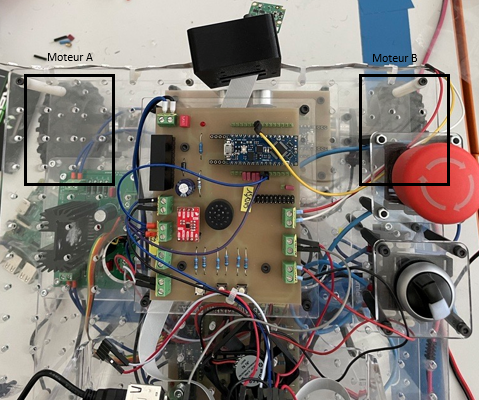
\includegraphics[scale=.8]{img/Haut_Robot.png}
	\vspace{.5cm}
	\label{img:img2}
	\captionabove{Positionnement des moteurs}
\end{figure}


\section{Graphiques}

\begin{center}
    

\begin{tikzpicture}
\pgfplotsset{every axis legend/.append style={
at={(0.5,1.03)},
anchor=north}}
\pgfplotstableread{Frequence250Hz_p30_i001_d0001_tick.prn}{\table}
\begin{axis}[
    xmin = 0, xmax = 180,
    ymin = 0, ymax = 70,
%    xtick distance = 1,
  %  ytick distance = 0.25,
    %grid = both,
   % minor tick num = 1,
   % major grid style = {lightgray},
   % minor grid style = {lightgray!25},
    width = \textwidth,
    height = 0.75\textwidth,
    %legend cell align = {left},
    %legend pos = north west
    legend columns = 4,
    xlabel = $ms$,
    ylabel = $tick/PWM$
]
 
\addplot[thick, blue] table [x = {x}, y = {y1}] {\table};
 
\addplot[thick, red] table [x ={x}, y = {y3}] {\table};
 
\addplot[thick, orange, smooth] table [x = {x}, y = {y2}] {\table};

\addplot[thick, brown, smooth] table [x = {x}, y = {y4}] {\table};

\legend{
    PWM Motor A,
    PWM Motor B,
    Tick A,
    Tick B,
}

\end{axis}
\label{graph:graph1} 
\end{tikzpicture}


\begin{itemize}
    \item Fréquence : 250Hz
    \item P : 30
    \item I : 0.01
    \item D : 0.001
    \item tours/s : 3
\end{itemize}
\end{center}

Ce premier graphe nous montre comment se comportait notre système avec les paramètres que nous avions choisi dans le cours 
du développement. On peut voir que le nombre de tick est toujours égal à 0 sauf lorsque les PWM tombent à 0. Là les ticks sont
à 1. C'est à partir de ce graphique que nous avons refait nos calculs pour qu'au minimum 3 ticks se fassent entre deux 
échantillonages par la fonction d'asservissement. \par

\begin{figure}[h]
    $\varnothing\ 90 = D$ \par
    $D \cdot \pi = P$ \par
    $90 \cdot 10^-3 \cdot \pi = 0.2827m$ \par
    $1 tour = 0.2827m$ \par
    $3 \cfrac{tour}{s} \cdot 3.6 = 0.8481\cfrac{m}{s} \cdot 3.6 = 3.05\cfrac{km}{h}$ \par
    Une roue compteuse possède 24 trous, donc 24 incrémentations par tour \par
    $24 \cdot 3 = 72$ \par
    $3 / 72 = 0.04s$ \par
    Pour être sûr d'avoir suffisamment de trous nous mettons une fréquence à 12.5Hz, donc $80ms$
    \caption{Équation du PID}
    \label{eq1}
\end{figure}

Nous avons donc changé la fréquence d'acquisition à 12.5Hz. Voici le graphe que nous avions avec nos paramètres : 

\begin{center}
    

    \begin{tikzpicture}
    \pgfplotsset{every axis legend/.append style={
    at={(0.5,1.03)},
    anchor=north}}
    \pgfplotstableread{Frequence12.5Hz_p30_i001_d0001_tick.prn}{\table}
    \begin{axis}[
        xmin = 0, xmax = 8000,
        ymin = 0, ymax = 70,
    %    xtick distance = 1,
      %  ytick distance = 0.25,
        %grid = both,
       % minor tick num = 1,
       % major grid style = {lightgray},
       % minor grid style = {lightgray!25},
        width = \textwidth,
        height = 0.75\textwidth,
        %legend cell align = {left},
        %legend pos = north west
        legend columns = 4,
        xlabel = $ms$,
        ylabel = $tick/PWM$
    ]
     
    \addplot[thick, blue] table [x = {x}, y = {y1}] {\table};
     
    \addplot[thick, red] table [x ={x}, y = {y3}] {\table};
     
    \addplot[thick, orange, smooth] table [x = {x}, y = {y2}] {\table};
    
    \addplot[thick, brown, smooth] table [x = {x}, y = {y4}] {\table};
    
    \legend{
        PWM Motor A,
        PWM Motor B,
        Tick A,
        Tick B,
    }
    
    \end{axis}
    \label{graph:graph1} 
    \end{tikzpicture}
    
    
    \begin{itemize}
        \item Fréquence : 12.5Hz
        \item P : 30
        \item I : 0.01
        \item D : 0.001
        \item tours/sec : 3
    \end{itemize}
    \end{center}

Le comportement du PID se rapproche de ce que nous souhaitons voir. Le nombre de tick moyen est 4, ce qui est raisonnable, 
en sachant que pour créer une parabole, nous avons besoin de 2 points minimum et plus est toujours mieux. À partir de ce 
graphique nous avons décidé de refaire notre cheminement pour obtenir un PID robuste. Le P est resté inchangé. \par

\begin{center}
    \begin{tikzpicture}
    \pgfplotsset{every axis legend/.append style={
    at={(0.5,1.03)},
    anchor=north}}
    \pgfplotstableread{Frequence12.5Hz_p30_i0.05_tick_4tours.prn}{\table}
    \begin{axis}[
        xmin = 0, xmax = 8000,
        ymin = 0, ymax = 150,
    %    xtick distance = 1,
      %  ytick distance = 0.25,
        %grid = both,
       % minor tick num = 1,
       % major grid style = {lightgray},
       % minor grid style = {lightgray!25},
        width = \textwidth,
        height = 0.75\textwidth,
        %legend cell align = {left},
        %legend pos = north west
        legend columns = 4,
        xlabel = $ms$,
        ylabel = $tick/PWM$
    ]
     
    \addplot[thick, blue] table [x = {x}, y = {y1}] {\table};
     
    \addplot[thick, red] table [x ={x}, y = {y3}] {\table};
     
    \addplot[thick, orange, smooth] table [x = {x}, y = {y2}] {\table};
    
    \addplot[thick, brown, smooth] table [x = {x}, y = {y4}] {\table};
    
    \legend{
        PWM Motor A,
        PWM Motor B,
        Tick A,
        Tick B,
    }
    
    \end{axis}
    \label{graph:graph1} 
    \end{tikzpicture}
    
    
    \begin{itemize}
        \item Fréquence : 12.5Hz
        \item P : 30
        \item I : 0.05
        \item tours/s : 4
    \end{itemize}
    \end{center}

    Nous avons changé quelques paramètres. Le I est à 0.05 et les tours/s sont de 4. On peut observer 
que ces sursauts de la part des PWM proviennent du I qui est trop grand pour le système à roue libre. 
Les 4 tours/s aident pour la vitesse de prise des données. Nous avons donc descendu le facteur I. \par

\begin{center}
    \begin{tikzpicture}
    \pgfplotsset{every axis legend/.append style={
    at={(0.5,1.03)},
    anchor=north}}
    \pgfplotstableread{Frequence12.5Hz_p30_i0.03_tick_4tours.prn}{\table}
    \begin{axis}[
        xmin = 0, xmax = 12000,
        ymin = 0, ymax = 150,
    %    xtick distance = 1,
      %  ytick distance = 0.25,
        %grid = both,
       % minor tick num = 1,
       % major grid style = {lightgray},
       % minor grid style = {lightgray!25},
        width = \textwidth,
        height = 0.75\textwidth,
        %legend cell align = {left},
        %legend pos = north west
        legend columns = 4,
        xlabel = $ms$,
        ylabel = $tick/PWM$
    ]
     
    \addplot[thick, blue] table [x = {x}, y = {y1}] {\table};
     
    \addplot[thick, red] table [x ={x}, y = {y3}] {\table};
     
    \addplot[thick, orange, smooth] table [x = {x}, y = {y2}] {\table};
    
    \addplot[thick, brown, smooth] table [x = {x}, y = {y4}] {\table};
    
    \legend{
        PWM Motor A,
        PWM Motor B,
        Tick A,
        Tick B,
    }
    
    \end{axis}
    \label{graph:graph1} 
    \end{tikzpicture}
    
    
    \begin{itemize}
        \item Fréquence : 12.5Hz
        \item P : 30
        \item I : 0.03
        \item tours/s : 4
    \end{itemize}
    \end{center}

Nous avons choisi ici de présenter une plus grande plage de données. En effet, ce que nous recherchons est la stabilisation du système. 
Nous l'avons après 10$s$. À partir de ce graphe nous avons essayé une valeur pour le D. \par

\begin{center}
    \begin{tikzpicture}
    \pgfplotsset{every axis legend/.append style={
    at={(0.5,1.03)},
    anchor=north}}
    \pgfplotstableread{Frequence12.5Hz_p30_i0.03_d2_tick_4tours.prn}{\table}
    \begin{axis}[
        xmin = 0, xmax = 8000,
        ymin = 0, ymax = 150,
    %    xtick distance = 1,
      %  ytick distance = 0.25,
        %grid = both,
       % minor tick num = 1,
       % major grid style = {lightgray},
       % minor grid style = {lightgray!25},
        width = \textwidth,
        height = 0.75\textwidth,
        %legend cell align = {left},
        %legend pos = north west
        legend columns = 4,
        xlabel = $ms$,
        ylabel = $tick/PWM$
    ]
     
    \addplot[thick, blue] table [x = {x}, y = {y1}] {\table};
     
    \addplot[thick, red] table [x ={x}, y = {y3}] {\table};
     
    \addplot[thick, orange, smooth] table [x = {x}, y = {y2}] {\table};
    
    \addplot[thick, brown, smooth] table [x = {x}, y = {y4}] {\table};
    
    \legend{
        PWM Motor A,
        PWM Motor B,
        Tick A,
        Tick B,
    }
    
    \end{axis}
    \label{graph:graph1} 
    \end{tikzpicture}
    
    
    \begin{itemize}
        \item Fréquence : 12.5Hz
        \item P : 30
        \item I : 0.03
        \item D : 2
        \item tours/s : 4
    \end{itemize}
    \end{center}

Nous voyons ci-dessus une stabilisation bien plus rapide avec le facteur D. Ce graphe nous est satisfaisant et nous passons sur les mêmes paramètres 
mais avec des frottements. Nous avons recommencé le même processus en sachant l'ordre de grandeur des différents facteurs dont nous aurons besoin 
grâce aux précédents graphiques. \par

Dans les prochains graphiques, nous allons surtout nous intéresser au fait que les courbes des ticks soient le plus similaire possible, ce qui se 
traduit par une vitesse sembable. \par

\begin{center}
    \begin{tikzpicture}
    \pgfplotsset{every axis legend/.append style={
    at={(0.5,1.03)},
    anchor=north}}
    \pgfplotstableread{12.5Hz_p30_4tours_F.prn}{\table}
    \begin{axis}[
        xmin = 0, xmax = 8000,
        ymin = 0, ymax = 150,
    %    xtick distance = 1,
      %  ytick distance = 0.25,
        %grid = both,
       % minor tick num = 1,
       % major grid style = {lightgray},
       % minor grid style = {lightgray!25},
        width = \textwidth,
        height = 0.75\textwidth,
        %legend cell align = {left},
        %legend pos = north west
        legend columns = 4,
        xlabel = $ms$,
        ylabel = $tick/PWM$
    ]
     
    \addplot[thick, blue] table [x = {x}, y = {y1}] {\table};
     
    \addplot[thick, red] table [x ={x}, y = {y3}] {\table};
     
    \addplot[thick, orange, smooth] table [x = {x}, y = {y2}] {\table};
    
    \addplot[thick, brown, smooth] table [x = {x}, y = {y4}] {\table};
    
    \legend{
        PWM Motor A,
        PWM Motor B,
        Tick A,
        Tick B,
    }
    
    \end{axis}
    \label{graph:graph1} 
    \end{tikzpicture}
    
    
    \begin{itemize}
        \item Fréquence : 12.5Hz
        \item P : 30
        \item Frottements
        \item 4 tours/s
    \end{itemize}
    \end{center}

Le comportement du robot observé était qu'il tournait sur lui-même dans le sens anti-horaire. Nous voyons que les courbes des PWM sont semblables, 
mais les ticks sont décalés. Le moteur B tournait plus vite que le moteur A. Nous allons voir le comportement avec le facteur I. \par

Le prochain graphique comporte beaucoup de changement. Nous avons ajouté 10 PWM pour le contrôleur du moteur A et changé la vitesse 
à 3 tours/s. Si c'était à refaire, nous ferions plus d'acquisition de données. Il y a un changement des conditions trop brusques. \par

\begin{center}
    \begin{tikzpicture}
    \pgfplotsset{every axis legend/.append style={
    at={(0.5,1.03)},
    anchor=north}}
    \pgfplotstableread{12.5Hz_p30_i0.01_m+10_3tours_F.prn}{\table}
    \begin{axis}[
        xmin = 0, xmax = 8000,
        ymin = 0, ymax = 200,
    %    xtick distance = 1,
      %  ytick distance = 0.25,
        %grid = both,
       % minor tick num = 1,
       % major grid style = {lightgray},
       % minor grid style = {lightgray!25},
        width = \textwidth,
        height = 0.75\textwidth,
        %legend cell align = {left},
        %legend pos = north west
        legend columns = 4,
        xlabel = $ms$,
        ylabel = $tick/PWM$
    ]
     
    \addplot[thick, blue] table [x = {x}, y = {y1}] {\table};
     
    \addplot[thick, red] table [x ={x}, y = {y3}] {\table};
     
    \addplot[thick, orange, smooth] table [x = {x}, y = {y2}] {\table};
    
    \addplot[thick, brown, smooth] table [x = {x}, y = {y4}] {\table};
    
    \legend{
        PWM Motor A,
        PWM Motor B,
        Tick A,
        Tick B,
    }
    
    \end{axis}
    \label{graph:graph1} 
    \end{tikzpicture}
    
    
    \begin{itemize}
        \item Fréquence : 12.5Hz
        \item P : 30
        \item I : 0.01
        \item Frottements
        \item 3 tours/s
        \item Moteur A + 10
    \end{itemize}
    \end{center}

Lors de ce test le robot a dû être replacé pour éviter un obstacle. Cela explique le changement brutal au milieu. Le robot a d'abord tourné à 
gauche, puis après le repositionnement à droite. On en déduit que la valeur ajoutée au moteur A est trop grande. Nous allons la changer ainsi 
que le nombre de tours et le facteur I qui reste encore trop abrupt. \par

\begin{center}
    \begin{tikzpicture}
    \pgfplotsset{every axis legend/.append style={
    at={(0.5,1.03)},
    anchor=north}}
    \pgfplotstableread{12.5Hz_p30_i0.001_m+5_4tours_F.prn}{\table}
    \begin{axis}[
        xmin = 0, xmax = 8000,
        ymin = 0, ymax = 200,
    %    xtick distance = 1,
      %  ytick distance = 0.25,
        %grid = both,
       % minor tick num = 1,
       % major grid style = {lightgray},
       % minor grid style = {lightgray!25},
        width = \textwidth,
        height = 0.75\textwidth,
        %legend cell align = {left},
        %legend pos = north west
        legend columns = 4,
        xlabel = $ms$,
        ylabel = $tick/PWM$
    ]
     
    \addplot[thick, blue] table [x = {x}, y = {y1}] {\table};
     
    \addplot[thick, red] table [x ={x}, y = {y3}] {\table};
     
    \addplot[thick, orange, smooth] table [x = {x}, y = {y2}] {\table};
    
    \addplot[thick, brown, smooth] table [x = {x}, y = {y4}] {\table};
    
    \legend{
        PWM Motor A,
        PWM Motor B,
        Tick A,
        Tick B,
    }
    
    \end{axis}
    \label{graph:graph1} 
    \end{tikzpicture}
    
    
    \begin{itemize}
        \item Fréquence : 12.5Hz
        \item P : 30
        \item I : 0.001
        \item Frottements
        \item 4 tours/s
        \item Moteur A + 5
    \end{itemize}
    \end{center}

Le robot a d'abord tourné sur la gauche, puis est rentré dans un obstacle. Après l'avoir reposé à terre, il est allé tout droit. 
On peut voir que les courbes des ticks se rejoignent bien après l'erreur du repositionnement. 
Nous nous approchons des valeurs qui nous permettraient d'avoir 
un robot qui avance tout droit. Cependant, on voit qu'il prend $4s$ pour que l'intégratif rende l'erreur 
presque nulle. \par

\begin{center}
    \begin{tikzpicture}
    \pgfplotsset{every axis legend/.append style={
    at={(0.5,1.03)},
    anchor=north}}
    \pgfplotstableread{12.5Hz_p30_i0.01_M+3_Ftrue.prn}{\table}
    \begin{axis}[
        xmin = 0, xmax = 8000,
        ymin = 0, ymax = 200,
    %    xtick distance = 1,
      %  ytick distance = 0.25,
        %grid = both,
       % minor tick num = 1,
       % major grid style = {lightgray},
       % minor grid style = {lightgray!25},
        width = \textwidth,
        height = 0.75\textwidth,
        %legend cell align = {left},
        %legend pos = north west
        legend columns = 4,
        xlabel = $ms$,
        ylabel = $tick/PWM$
    ]
     
    \addplot[thick, blue] table [x = {x}, y = {y1}] {\table};
     
    \addplot[thick, red] table [x ={x}, y = {y3}] {\table};
     
    \addplot[thick, orange, smooth] table [x = {x}, y = {y2}] {\table};
    
    \addplot[thick, brown, smooth] table [x = {x}, y = {y4}] {\table};
    
    \legend{
        PWM Motor A,
        PWM Motor B,
        Tick A,
        Tick B,
    }
    
    \end{axis}
    \label{graph:graph1} 
    \end{tikzpicture}
    
    
    \begin{itemize}
        \item Fréquence : 12.5Hz
        \item P : 30
        \item I : 0.01
        \item Frottements
        \item 4 tours/s
        \item Moteur A + 3
    \end{itemize}
    \end{center}

    Le robot a d'abord tourné à gauche, ensuite tout droit, puis à droite 
    et est rentré dans un mur. Nous allons essayer de
    rajouter le D pour voir s'il permet de combler 
    l'incrémentation du moteur. \par

    \begin{center}
        \begin{tikzpicture}
        \pgfplotsset{every axis legend/.append style={
        at={(0.5,1.03)},
        anchor=north}}
        \pgfplotstableread{12.5Hz_p30_i0.01_d2_F.prn}{\table}
        \begin{axis}[
            xmin = 0, xmax = 8000,
            ymin = 0, ymax = 200,
        %    xtick distance = 1,
          %  ytick distance = 0.25,
            %grid = both,
           % minor tick num = 1,
           % major grid style = {lightgray},
           % minor grid style = {lightgray!25},
            width = \textwidth,
            height = 0.75\textwidth,
            %legend cell align = {left},
            %legend pos = north west
            legend columns = 4,
            xlabel = $ms$,
            ylabel = $tick/PWM$
        ]
         
        \addplot[thick, blue] table [x = {x}, y = {y1}] {\table};
         
        \addplot[thick, red] table [x ={x}, y = {y3}] {\table};
         
        \addplot[thick, orange, smooth] table [x = {x}, y = {y2}] {\table};
        
        \addplot[thick, brown, smooth] table [x = {x}, y = {y4}] {\table};
        
        \legend{
            PWM Motor A,
            PWM Motor B,
            Tick A,
            Tick B,
        }
        
        \end{axis}
        \label{graph:graph1} 
        \end{tikzpicture}
        
        
        \begin{itemize}
            \item Fréquence : 12.5Hz
            \item P : 30
            \item I : 0.01
            \item D : 2
            \item Frottements
            \item 4 tours/s
        \end{itemize}
        \end{center}

Le robot a d'abord tourné à gauche puis puis tout droit et 
enfin à droite. Pour voir exactement si le facteur I
est trop petit nous avons essayé de le mettre à 1. \par

\begin{center}
    \begin{tikzpicture}
    \pgfplotsset{every axis legend/.append style={
    at={(0.5,1.03)},
    anchor=north}}
    \pgfplotstableread{12.5Hz_p30_i1_d2_F.prn}{\table}
    \begin{axis}[
        xmin = 0, xmax = 8000,
        ymin = 0, ymax = 260,
    %    xtick distance = 1,
      %  ytick distance = 0.25,
        %grid = both,
       % minor tick num = 1,
       % major grid style = {lightgray},
       % minor grid style = {lightgray!25},
        width = \textwidth,
        height = 0.75\textwidth,
        %legend cell align = {left},
        %legend pos = north west
        legend columns = 4,
        xlabel = $ms$,
        ylabel = $tick/PWM$
    ]
     
    \addplot[thick, blue] table [x = {x}, y = {y1}] {\table};
     
    \addplot[thick, red] table [x ={x}, y = {y3}] {\table};
     
    \addplot[thick, orange, smooth] table [x = {x}, y = {y2}] {\table};
    
    \addplot[thick, brown, smooth] table [x = {x}, y = {y4}] {\table};
    
    \legend{
        PWM Motor A,
        PWM Motor B,
        Tick A,
        Tick B,
    }
    
    \end{axis}
    \label{graph:graph1} 
    \end{tikzpicture}
    
    
    \begin{itemize}
        \item Fréquence : 12.5Hz
        \item P : 30
        \item I : 1
        \item D : 2
        \item Frottements
        \item 4 tours/s
    \end{itemize}
    \end{center}

On peut observer que le comportement du robot était 
erratique. Il faisait drift sur drift en tournant sur lui-même. 
Nous allons essayer de descendre le facteur P pour qu'il y ait moins d'erreur
à intégrer. \par

\begin{center}
    \begin{tikzpicture}
    \pgfplotsset{every axis legend/.append style={
    at={(0.5,1.03)},
    anchor=north}}
    \pgfplotstableread{12.5Hz_p5_i1_d2_F.prn}{\table}
    \begin{axis}[
        xmin = 0, xmax = 8000,
        ymin = 0, ymax = 260,
    %    xtick distance = 1,
      %  ytick distance = 0.25,
        %grid = both,
       % minor tick num = 1,
       % major grid style = {lightgray},
       % minor grid style = {lightgray!25},
        width = \textwidth,
        height = 0.75\textwidth,
        %legend cell align = {left},
        %legend pos = north west
        legend columns = 4,
        xlabel = $ms$,
        ylabel = $tick/PWM$
    ]
     
    \addplot[thick, blue] table [x = {x}, y = {y1}] {\table};
     
    \addplot[thick, red] table [x ={x}, y = {y3}] {\table};
     
    \addplot[thick, orange, smooth] table [x = {x}, y = {y2}] {\table};
    
    \addplot[thick, brown, smooth] table [x = {x}, y = {y4}] {\table};
    
    \legend{
        PWM Motor A,
        PWM Motor B,
        Tick A,
        Tick B,
    }
    
    \end{axis}
    \label{graph:graph1} 
    \end{tikzpicture}
    
    
    \begin{itemize}
        \item Fréquence : 12.5Hz
        \item P : 5
        \item I : 1
        \item D : 2
        \item Frottements
        \item 4 tours/s
    \end{itemize}
    \end{center}

Pour avoir des données traitables, nous allons descendre le facteur I. \par

\begin{center}
    \begin{tikzpicture}
    \pgfplotsset{every axis legend/.append style={
    at={(0.5,1.03)},
    anchor=north}}
    \pgfplotstableread{12.5Hz_p5_i0.01_d2_F.prn}{\table}
    \begin{axis}[
        xmin = 0, xmax = 8000,
        ymin = 0, ymax = 260,
    %    xtick distance = 1,
      %  ytick distance = 0.25,
        %grid = both,
       % minor tick num = 1,
       % major grid style = {lightgray},
       % minor grid style = {lightgray!25},
        width = \textwidth,
        height = 0.75\textwidth,
        %legend cell align = {left},
        %legend pos = north west
        legend columns = 4,
        xlabel = $ms$,
        ylabel = $tick/PWM$
    ]
     
    \addplot[thick, blue] table [x = {x}, y = {y1}] {\table};
     
    \addplot[thick, red] table [x ={x}, y = {y3}] {\table};
     
    \addplot[thick, orange, smooth] table [x = {x}, y = {y2}] {\table};
    
    \addplot[thick, brown, smooth] table [x = {x}, y = {y4}] {\table};
    
    \legend{
        PWM Motor A,
        PWM Motor B,
        Tick A,
        Tick B,
    }
    
    \end{axis}
    \label{graph:graph1} 
    \end{tikzpicture}
    
    
    \begin{itemize}
        \item Fréquence : 12.5Hz
        \item P : 5
        \item I : 0.01
        \item D : 2
        \item Frottements
        \item 4 tours/s
    \end{itemize}
    \end{center}

Cette fois-ci, nous allons enlever le facteur D. Nous allons 
aussi plafonner à 160 les PWM. \par

\begin{center}
    \begin{tikzpicture}
    \pgfplotsset{every axis legend/.append style={
    at={(0.5,1.03)},
    anchor=north}}
    \pgfplotstableread{12.5Hz_p5_i0.08_MAX160_F.prn}{\table}
    \begin{axis}[
        xmin = 0, xmax = 8000,
        ymin = 0, ymax = 260,
    %    xtick distance = 1,
      %  ytick distance = 0.25,
        %grid = both,
       % minor tick num = 1,
       % major grid style = {lightgray},
       % minor grid style = {lightgray!25},
        width = \textwidth,
        height = 0.75\textwidth,
        %legend cell align = {left},
        %legend pos = north west
        legend columns = 4,
        xlabel = $ms$,
        ylabel = $tick/PWM$
    ]
     
    \addplot[thick, blue] table [x = {x}, y = {y1}] {\table};
     
    \addplot[thick, red] table [x ={x}, y = {y3}] {\table};
     
    \addplot[thick, orange, smooth] table [x = {x}, y = {y2}] {\table};
    
    \addplot[thick, brown, smooth] table [x = {x}, y = {y4}] {\table};
    
    \legend{
        PWM Motor A,
        PWM Motor B,
        Tick A,
        Tick B,
    }
    
    \end{axis}
    \label{graph:graph1} 
    \end{tikzpicture}
    
    
    \begin{itemize}
        \item Fréquence : 12.5Hz
        \item P : 5
        \item I : 0.01
        \item MAX : 160
        \item Frottements
        \item 4 tours/s
    \end{itemize}
    \end{center}

Nous pouvons voir qu'un seul moteur a eu une limite, faute de notre part. 
Nous allons aussi mettre un maximum à 200. Cependant, la courbe du 
moteur B est très intéressante. La prochaine séance de test sera dirigé 
vers elle. \par

\begin{center}
    \begin{tikzpicture}
    \pgfplotsset{every axis legend/.append style={
    at={(0.5,1.03)},
    anchor=north}}
    \pgfplotstableread{12.5Hz_p3_i0.08_MAX200_F.prn}{\table}
    \begin{axis}[
        xmin = 0, xmax = 8000,
        ymin = 0, ymax = 260,
    %    xtick distance = 1,
      %  ytick distance = 0.25,
        %grid = both,
       % minor tick num = 1,
       % major grid style = {lightgray},
       % minor grid style = {lightgray!25},
        width = \textwidth,
        height = 0.75\textwidth,
        %legend cell align = {left},
        %legend pos = north west
        legend columns = 4,
        xlabel = $ms$,
        ylabel = $tick/PWM$
    ]
     
    \addplot[thick, blue] table [x = {x}, y = {y1}] {\table};
     
    \addplot[thick, red] table [x ={x}, y = {y3}] {\table};
     
    \addplot[thick, orange, smooth] table [x = {x}, y = {y2}] {\table};
    
    \addplot[thick, brown, smooth] table [x = {x}, y = {y4}] {\table};
    
    \legend{
        PWM Motor A,
        PWM Motor B,
        Tick A,
        Tick B,
    }
    
    \end{axis}
    \label{graph:graph1} 
    \end{tikzpicture}
    
    
    \begin{itemize}
        \item Fréquence : 12.5Hz
        \item P : 3
        \item I : 0.01
        \item MAX : 200
        \item Frottements
        \item 4 tours/s
    \end{itemize}
    \end{center}

Honnêtement, le graphique est juste étrange. Je pense descendre la valeur 
du I encore plus. Ce qui serait intéressant est d'avoir la consigne et la valeur 
mesurée, essayer pour les prochains graphiques. \par

Dans les prochains graphiques, nous aurons les vitesses observées ainsi que leur 
consigne tout en gardant les PWM. \par

\begin{center}
    \begin{tikzpicture}
    \pgfplotsset{every axis legend/.append style={
    at={(0.5,1.03)},
    anchor=north}}
    \pgfplotstableread{12.5Hz_p2_i0.01_F.prn}{\table}
    \begin{axis}[
        xmin = 0, xmax = 8000,
        ymin = 0, ymax = 10,
    %    xtick distance = 1,
      %  ytick distance = 0.25,
        %grid = both,
       % minor tick num = 1,
       % major grid style = {lightgray},
       % minor grid style = {lightgray!25},
        width = \textwidth,
        height = 0.75\textwidth,
        %legend cell align = {left},
        %legend pos = north west
        legend columns = 3,
        xlabel = $ms$,
        ylabel = $\cfrac{tours}{s}$]
    
     

     
    \addplot[thick, blue] table [x = {x}, y = {y2}] {\table};
    
    \addplot[thick, red] table [x = {x}, y = {y4}] {\table};

    \addplot[thick, green, smooth] table [x = {x}, y = {y5}] {\table};
    
    \legend{
        vitesse moteur A,
        vitesse moteur B,
        Consigne,}
    
    \end{axis}
    \label{graph:graph1} 
    \end{tikzpicture}
    
    
    \begin{itemize}
        \item Fréquence : 12.5Hz
        \item P : 2
        \item I : 0.01
        \item Frottements
        \item 4 tours/s
    \end{itemize}
    \end{center}

Le robot tournait encore beaucoup, j'ai décidé de réduire encore le P et le I. \par

\begin{center}
    \begin{tikzpicture}
    \pgfplotsset{every axis legend/.append style={
    at={(0.5,1.03)},
    anchor=north}}
    \pgfplotstableread{12.5Hz_p0.85_i0.01_F.prn}{\table}
    \begin{axis}[
        xmin = 0, xmax = 8000,
        ymin = 0, ymax = 10,
    %    xtick distance = 1,
      %  ytick distance = 0.25,
        %grid = both,
       % minor tick num = 1,
       % major grid style = {lightgray},
       % minor grid style = {lightgray!25},
        width = \textwidth,
        height = 0.75\textwidth,
        %legend cell align = {left},
        %legend pos = north west
        legend columns = 3,
        xlabel = $ms$,
        ylabel = $\cfrac{tours}{s}$]
    
     

     
    \addplot[thick, blue] table [x = {x}, y = {y2}] {\table};
    
    \addplot[thick, red] table [x = {x}, y = {y4}] {\table};

    \addplot[thick, green, smooth] table [x = {x}, y = {y5}] {\table};
    
    \legend{
        vitesse moteur A,
        vitesse moteur B,
        Consigne,}
    
    \end{axis}
    \label{graph:graph1} 
    \end{tikzpicture}
    
    
    \begin{itemize}
        \item Fréquence : 12.5Hz
        \item P : 0.85
        \item I : 0.01
        \item Frottements
        \item 4 tours/s
    \end{itemize}
    \end{center}

Le robot est allé droit sur plus de 5m. La victoire est proche.
Nous devrions revoir notre calcul de vitesse qu'il se fasse en $int$
uniquement avec les ticks. Descendre le I permettrait d'amener 
un meilleur contrôle du robot. \par


\chapter{Conclusion}



\end{document}